\section{Alternative modeling of QKD}
\label{sec:alternative}

So far we discussed QKD as protocols that start with an insecure
quantum channel and an authentic classical channel and generate, as
the desired ideal resource, a key of fixed length. In this section we
discuss other variants of QKD protocols, where these resources are
chosen differently. In \secref{sec:alternative.adaptive} we
consider an ideal key resource with adaptive key length. In
\secref{sec:alternative.entanglement} we discuss protocols which
use a source of entanglement instead of an insecure quantum
channel. In \secref{sec:alternative.randomness} we show how to
model a situation in which no perfect randomness is available.  In
\secref{sec:alternative.di} we model device\-/independent
QKD. Relaxations of this known as semi\-/device\-/independence are
discussed in \secref{sec:alternative.semi}. Finally, in
\secref{sec:alternative.memoryless} we consider adversaries that have
no quantum memory.


\subsection{Adaptive key length}
\label{sec:alternative.adaptive}

For a protocol to construct the shared secret key resource of \figref{fig:qkd.resource.switch}, it must either abort or produce a key of a fixed length. A more practical protocol could adapt the secret key length to the noise level of the quantum channel. This provides the adversary with the functionality to control the key length (not only whether it gets generated or not), and can be modeled by allowing the key length to be input at Eve's interface of the ideal key resource, as illustrated in \figref{fig:qkd.resource.adaptive}.

\begin{figure}[tb]


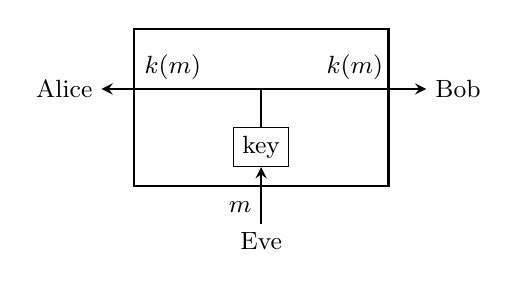
\begin{tikzpicture}[
sArrow/.style={->,>=stealth,thick},
largeResource/.style={draw,thick,minimum width=1.618*2cm,minimum height=2cm}]

\small

\def\u{.236} %2/1.618-1

\node[largeResource] (keyBox) at (0,0) {};
\node (alice) at (-2.5,\u) {Alice};
\node (bob) at (2.5,\u) {Bob};
\node (eve) at (0,-1.7) {Eve};
\node[draw] (key) at (0,-.5) {key};

\draw[sArrow,<->] (alice) to node[pos=.22,auto] {$k(m)$} node[pos=.78,auto] {$k(m)$} (bob);
\draw[thick] (0,\u) to (key);
\draw[sArrow] (eve) to node[pos=.3,auto] {$m$} (key);

\end{tikzpicture}

\caption[Secret key resource with adaptive
length]{\label{fig:qkd.resource.adaptive}A secret key resource with   adaptive key length. This resources allows Eve to choose the length $m$   of the final key $k$, which is then output at Alice's and Bob's interfaces.}
\end{figure}

Such an ideal resource has been considered in \textcite{BHLMO05,HT12}. The reduction from the corresponding security definition in AC to a trace distance criterion still goes through. But instead of \eqnref{eq:d}, we get 
\begin{equation} \label{eq:adpative.trace.d}
\sum_m p_m D \left( \rho^m_{KE},\tau^m_K \otimes \rho^m_E \right) \leq
\eps,
\end{equation}
where $p_m$ is the probability of obtaining a key of length $m$, $\rho^m_{KE}$ is the joint state of the key and Eve's system conditioned on the key having length $m$,  and $\tau^m_K$ is a fully mixed state of dimension $2^m$.


\subsection{Source of entanglement}
\label{sec:alternative.entanglement}

In contrast to \emph{prepare\-/and\-/measure} protocols,
\emph{entanglement\-/based} protocols, e.g., \textcite{Eke91,BBM92},
use a source of entanglement, instead of a quantum communication
channel. It is also pretty standard in security proofs to first
transform a given prepare\-/and\-/measure protocol into an
entanglement\-/based one, and then prove the security of the
latter~\cite{SP00}. In \figref{fig:qkd.real.ent} we draw the system
consisting of a QKD protocol $(\pi^{\qkd}_A,\pi^{\qkd}_B)$, the
authentic channel $\aA$ and a source  $\aE$ of entangled states, which may be
controlled by Eve. To specify the completeness property, we also consider
a source of entanglement $\aE'$ that produces a fixed bipartite
entangled state instead of allowing Eve to decide.

\begin{figure}[tb]


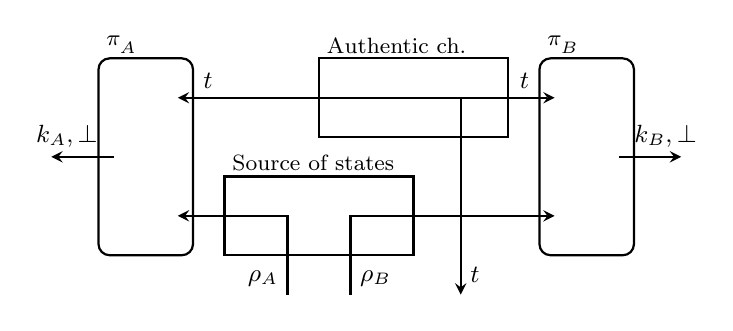
\begin{tikzpicture}[
sArrow/.style={->,>=stealth,thick},
thinResource/.style={draw,thick,minimum width=2.4cm,minimum height=1cm},
protocol/.style={draw,rounded corners,thick,minimum width=1.2cm,minimum height=2.5cm},
pnode/.style={minimum width=.8cm,minimum height=.5cm}]

\small

\def\t{4} %.6+1.2+.4+1.2*3/2
\def\u{2.8} %1.2/2+.4+1.2*3/2
\def\v{.75}
\def\w{.6} %1.2/2

\node[pnode] (a1) at (-\u,\v) {};
\node[pnode] (a2) at (-\u,0) {};
\node[pnode] (a3) at (-\u,-\v) {};
\node[protocol] (a) at (-\u,0) {};
\node[yshift=-2,above right] at (a.north west) {\footnotesize
  $\pi^{\qkd}_A$};
\node (alice) at (-\t,0) {};

\node[pnode] (b1) at (\u,\v) {};
\node[pnode] (b2) at (\u,0) {};
\node[pnode] (b3) at (\u,-\v) {};
\node[protocol] (b) at (\u,0) {};
\node[yshift=-2,above right] at (b.north west) {\footnotesize $\pi^{\qkd}_B$};
\node (bob) at (\t,0) {};

\node[thinResource] (cch) at (\w,\v) {};
\node[yshift=-2,above right] at (cch.north west) {\footnotesize
  Authentic ch.~$\aA$};
\node[thinResource] (qch) at (-\w,-\v) {};
\node[yshift=-1.5,above right] at (qch.north west) {\footnotesize
  Source of states $\aE$};
\node (eveq1) at (-\w-.4,-1.75) {};
\node (junc1) at (eveq1 |- a3) {};
\node (eveq2) at (-\w+.4,-1.75) {};
\node (junc2) at (eveq2 |- a3) {};
\node (evec) at (\w+\w,-1.75) {};
\node (junc3) at (evec |- b1) {};

\draw[sArrow,<->] (a1) to node[auto,pos=.08] {$t$} node[auto,pos=.92] {$t$}  (b1);
\draw[sArrow] (junc3.center) to node[auto,pos=.9] {$t$} (evec.center);

\draw[sArrow] (a2) to node[auto,pos=.75,swap] {$k_{A},\bot$} (alice.center);
\draw[sArrow] (b2) to node[auto,pos=.75] {$k_{B},\bot$} (bob.center);

\draw[sArrow,<-] (a3) to (junc1.center) to node[pos=.8,auto,swap] {$\rho_A$} (eveq1.center);
\draw[sArrow] (eveq2.center) to node[pos=.2,auto,swap] {$\rho_B$} (junc2.center) to (b3);

\end{tikzpicture}


\caption[QKD system with source of
entanglement]{\label{fig:qkd.real.ent}A real QKD system that uses a
  source of entangled states. Instead of having access to an insecure
  channel as in \figref{fig:qkd.real.adv}, Alice and Bob use a source
  of entanglement $\aE$ that is controlled by Eve. This means that Eve may
  generate an arbitrary state $\rho_{ABE}$ of which the $A$ register goes to Alice and
  the $B$ register to Bob.}
\end{figure}

The reduction from the AC security definition to the trace distance criterion described in \secref{sec:security} works here, too, with the source of entanglement replacing the insecure channel, resulting in the same conditions for $\eps$\=/secrecy and $\eps$\=/correctness.

One can also show that any protocol designed for a distributed source
of entanglement can be transformed into one where a state is prepared
locally and sent over an (insecure) channel. To explain this, we first
decompose Alice's QKD protocol in two parts.  In the first she carries
out a subprotocol $\alpha$ that performs a measurement
$\bM^a = \{M^a_x\}_x$ on the state received from the source of
entangled states, where $\bM^a$ is chosen with some probability $p_a$
from a set $\{\bM^a\}_a$. The second part consists of the rest of her
QKD protocol. We illustrate this in \figref{fig:qkd.ent.protocol}.

\begin{figure}[tb]


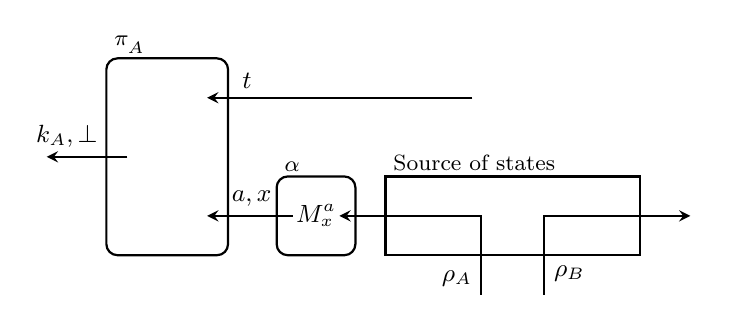
\begin{tikzpicture}[
sArrow/.style={->,>=stealth,thick},
thinResource/.style={draw,thick,minimum width=1.618*2cm,minimum height=1cm},
protocol/.style={draw,rounded corners,thick,minimum width=1.545cm,minimum height=2.5cm},
pnode/.style={minimum width=1cm,minimum height=.5cm},
sqResource/.style={draw,rounded corners,thick,minimum width=1cm,minimum height=1cm}]

\small

\def\t{5.92} %.75+1.545+.5+1+.5+1.618
\def\u{4.39} %1.545/2+.5+1+.5+1.618
\def\um{2.5} %1/2+.5+1.618-.1
\def\ub{2.37} %1.618+.75
\def\v{.75}


\node[pnode] (a1) at (-\u,\v) {};
\node[pnode] (a2) at (-\u,0) {};
\node[pnode] (a3) at (-\u,-\v) {};
\node[protocol] (a) at (-\u,0) {};
\node[yshift=-2,above right] at (a.north west) {\footnotesize
  $\pi^{\qkd}_A$};
\node (alice) at (-\t,0) {};

\node (b1) at (-.4,0 |- a1) {};
\node (b3) at (\ub,-\v) {};

\node[sqResource] (m) at (-\um,-\v) {};
\node[inner sep=1] (mInner) at (-\um,-\v) {$M^a_x$};
\node[yshift=-2,above right] at (m.north west) {\footnotesize
  $\alpha$};

\node[thinResource] (qch) at (0,-\v) {};
\node[yshift=-1.5,above right] at (qch.north west) {\footnotesize
  Source of states $\aE$};
\node (eveq1) at (-.4,-1.75) {};
\node (junc1) at (eveq1 |- a3) {};
\node (eveq2) at (.4,-1.75) {};
\node (junc2) at (eveq2 |- a3) {};

\draw[sArrow] (b1) to node[auto,pos=.85,swap] {$t$}  (a1);

\draw[sArrow] (a2) to node[auto,pos=.75,swap] {$k_{A},\bot$} (alice.center);

\draw[sArrow] (mInner) to node[swap,auto,pos=.48] {$a,x$} (a3);
\draw[sArrow,<-] (mInner) to (junc1.center) to node[pos=.8,auto,swap] {$\rho_A$} (eveq1.center);
\draw[sArrow] (eveq2.center) to node[pos=.264,auto,swap] {$\rho_B$} (junc2.center) to (b3);

\end{tikzpicture}


\caption[Entanglement based QKD
protocol]{\label{fig:qkd.ent.protocol}We split Alice's part of an
  entanglement\-/based QKD protocol in two parts, the measurement of
  the incoming states (denoted by $\alpha$) and the rest of the
  protocol (denoted by $\pi^{\qkd}_A$).}
\end{figure}

We now need to argue that there exists a converter $\gamma$ which constructs
$\alpha \aE$ from an insecure channel $\aQ$ and $\alpha \aE'$ from a
noiseless channel $\aQ'$. For this, we must
establish the two following conditions.
\begin{enumerate}[label=(\roman*), ref=\roman*]
\item \label{eq:ent.sec} There exists a simulator $\sigma_E$ such that
  \[ 
   \gamma \aQ = \alpha \aE \sigma_E.
\]
\item \label{eq:ent.cor} The following equality holds,
  \[\gamma \aQ' = \alpha \aE'.\] 
\end{enumerate}
Once we have established these conditions, it follows immediately from
the composition theorem of the AC framework~\cite{MR11} that any QKD
protocol which is sound when using $\alpha\aE$ and complete when using
$\alpha\aE'$ is also sound and complete when using $\gamma\aQ$ and
$\gamma\aQ'$, respectively.

Let $\rho_{AB}$ be the bipartite entangled state that is generated by
$\aE'$. Let
$\tilde{\varphi}^{x,a}_B \coloneqq \trace[A]{M^a_x \rho_{AB}
  \hconj{\left(M^a_x\right)}}$,
$p_{x|a} \coloneqq \tr \tilde{\varphi}^{x,a}_B$ and
$\varphi^{x,a}_B \coloneqq \tilde{\varphi}^{x,a}_B/p_{x|a}$. We define
the converter $\gamma$ to prepare the state $\varphi^{x,a}_B$ with
probability $p_ap_{x|a}$, which it sends on the insecure
channel. Furthermore, we define the simulator $\sigma_E$ to prepare
$\rho_{AB}$, input the $A$\=/part on the entanglement resource for
Alice and output the $B$\=/part at the outer interface. It is then
straightforward to check from \figref{fig:qkd.ent} that this satisfies
the conditions \eqref{eq:ent.sec} and \eqref{eq:ent.cor} described above.


\begin{figure*}[htb]
\centering
\subfloat[Soundness][\label{fig:qkd.ent.soundness}When modeling
  soundness, the adversary can modify the messages on the insecure
  channel $\aQ$. The simulator $\sigma_E$ generates the entangled state
  $\rho_{AB}$ that is expected from of a non\-/adversarial source of
  entangled states, and outputs the $B$ part at the outer interface,
  making the two systems on the left and right indistinguishable.]{
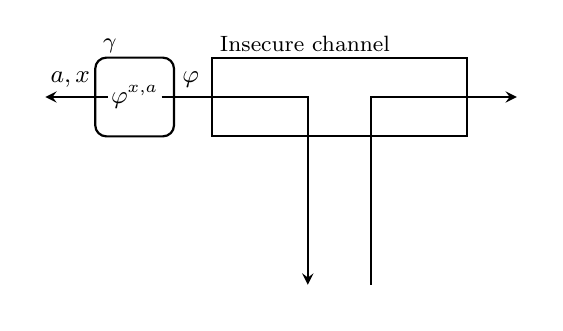
\begin{tikzpicture}[
sArrow/.style={->,>=stealth,thick},
thinResource/.style={draw,thick,minimum width=1.618*2cm,minimum height=1cm},
sqResource/.style={draw,rounded corners,thick,minimum width=1cm,minimum height=1cm}]

\small

\def\ua{3.85} %.75+1+.5+1.618
\def\um{2.6} %1/2+.5+1.618
\def\ub{2.37} %1.618+.75
\def\t{2.5}

\node (a) at (-\ua,0) {};
\node (b) at (\ub,0) {};

\node[sqResource] (m) at (-\um,0) {};
\node[inner sep=1] (mInner) at (-\um,0) {$\varphi^{x,a}$};
\node[yshift=-2,above right] at (m.north west) {\footnotesize
  $\gamma$};

\node[thinResource] (qch) at (0,0) {};
\node[yshift=-1.5,above right] at (qch.north west) {\footnotesize
  Insecure channel $\aQ$};

\node (le) at (-.4,-\t) {};
\node (re) at (.4,-\t) {};

\node (junc1) at (le |- a) {};
\node (junc2) at (re |- a) {};

\draw[sArrow] (mInner) to node[swap,auto,pos=.6] {$a,x$} (a);

\draw[sArrow] (mInner) to node[auto,pos=.2] {$\varphi$} (junc1.center) to (le);
\draw[sArrow] (re) to (junc2.center) to (b);

\end{tikzpicture}  \hspace{2cm}
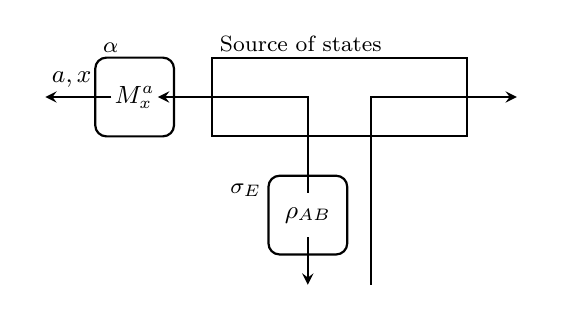
\begin{tikzpicture}[
sArrow/.style={->,>=stealth,thick},
thinResource/.style={draw,thick,minimum width=1.618*2cm,minimum height=1cm},
sqResource/.style={draw,rounded corners,thick,minimum width=1cm,minimum height=1cm}]

\small

\def\ua{3.85} %.75+1+.5+1.618
\def\um{2.6} %1/2+.5+1.618
\def\ub{2.37} %1.618+.75
\def\v{.75}
\def\t{2.5}

\node (a) at (-\ua,0) {};
\node (b) at (\ub,0) {};

\node[sqResource] (m) at (-\um,0) {};
\node[inner sep=1] (mInner) at (-\um,0) {$M^a_x$};
\node[yshift=-2,above right] at (m.north west) {\footnotesize
  $\alpha$};

\node[thinResource] (qch) at (0,0) {};
\node[yshift=-1.5,above right] at (qch.north west) {\footnotesize
  Source of states $\aE$};

\node[sqResource] (sim) at (-.4,-2*\v) {};
\node[inner sep=5] (simInner) at (-.4,-2*\v) {$\rho_{AB}$};
\node[xshift=1,below left] at (sim.north west) {\footnotesize $\sigma_E$};

\node (le) at (-.4,-\t) {};
\node (re) at (.4,-\t) {};

\node (junc1) at (le |- a) {};
\node (junc2) at (re |- a) {};

\draw[sArrow] (mInner) to node[swap,auto,pos=.6] {$a,x$} (a);

\draw[sArrow,<-] (mInner) to (junc1.center) to (simInner);
\draw[sArrow] (simInner) to (le);
\draw[sArrow] (re) to (junc2.center) to (b);

\end{tikzpicture}}

\vspace{12pt}

\subfloat[Completeness][\label{fig:qkd.ent.completeness}When modeling
completeness, the source of entanglement $\aE'$ prepares the state
$\rho_{AB}$. The systems on the left and right are
indistinguishable.]{
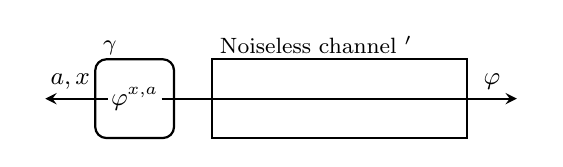
\begin{tikzpicture}[
sArrow/.style={->,>=stealth,thick},
thinResource/.style={draw,thick,minimum width=1.618*2cm,minimum height=1cm},
% filter/.style={draw,thick,minimum width=1.618cm,minimum height=1cm},
sqResource/.style={draw,rounded corners,thick,minimum width=1cm,minimum height=1cm}]

\small

\def\ua{3.85} %.75+1+.5+1.618
\def\um{2.6} %1/2+.5+1.618
\def\ub{2.37} %1.618+.75
\def\v{.75}

\node (a) at (-\ua,0) {};
\node (b) at (\ub,0) {};

\node[sqResource] (m) at (-\um,0) {};
\node[inner sep=1] (mInner) at (-\um,0) {$\varphi^{x,a}$};
\node[yshift=-2,above right] at (m.north west) {\footnotesize
  $\gamma$};

\node[thinResource] (qch) at (0,0) {};
\node[yshift=-1.5,above right] at (qch.north west) {\footnotesize
  Noiseless channel $\aQ'$};

% \node[filter] (qchf) at (0,-2*\v) {};
% \node[xshift=2,below left] at (qchf.north west) {\footnotesize $\sharp_E$};

% \node[xshift=-.4cm] (qchfl) at (qchf.center) {};
% \node[xshift=.4cm] (qchfr) at (qchf.center) {};
% \node (qchl) at (qchfl |- qchf.north) {};
% \node (qchr) at (qchfr |- qchf.north) {};
% \node (junc1) at (qchfl |- a) {};
% \node (junc2) at (qchfr |- a) {};

\draw[sArrow] (mInner) to node[swap,auto,pos=.6] {$a,x$} (a);

\draw[sArrow] (mInner) to node[auto,pos=.93] {$\varphi$} (b);

% \draw[sArrow] (qchl.center) to (qchfl.center) to (qchfr.center) to (qchr.center);

\end{tikzpicture} \hspace{2cm}
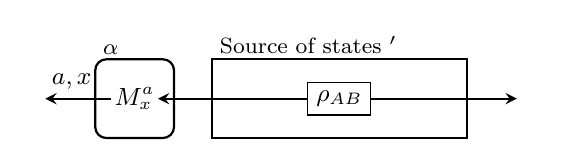
\begin{tikzpicture}[
sArrow/.style={->,>=stealth,thick},
thinResource/.style={draw,thick,minimum width=1.618*2cm,minimum height=1cm},
% filter/.style={draw,thick,minimum width=1.618cm,minimum height=1cm},
sqResource/.style={draw,rounded corners,thick,minimum width=1cm,minimum height=1cm}]

\small

\def\ua{3.85} %.75+1+.5+1.618
\def\um{2.6} %1/2+.5+1.618
\def\ub{2.37} %1.618+.75
\def\v{.75}

\node (a) at (-\ua,0) {};
\node (b) at (\ub,0) {};

\node[sqResource] (m) at (-\um,0) {};
\node[inner sep=1] (mInner) at (-\um,0) {$M^a_x$};
\node[yshift=-2,above right] at (m.north west) {\footnotesize
  $\alpha$};

\node[thinResource] (qch) at (0,0) {};
\node[yshift=-1.5,above right] at (qch.north west) {\footnotesize
  Source of states $\aE'$};

% \node[filter] (qchf) at (0,-2*\v) {};
% \node[xshift=2,below left] at (qchf.north west) {\footnotesize $\lozenge_E$};
\node[draw] (boxState) at (0,0) {$\rho_{AB}$};

% \node[xshift=-.4cm] (qchfl) at (qchf.center) {};
% \node[xshift=.4cm] (qchfr) at (qchf.center) {};
% \node (qchl) at (qchfl |- qchf.north) {};
% \node (qchr) at (qchfr |- qchf.north) {};
% \node (junc1) at (qchfl |- a) {};
% \node (junc2) at (qchfr |- a) {};

\draw[sArrow] (mInner) to node[swap,auto,pos=.6] {$a,x$} (a);

\draw[sArrow] (boxState) to (mInner);
\draw[sArrow] (boxState) to (b);

% \draw[sArrow,<->] (qchl.center) to (qchfl.center) to (qchfr.center) to (qchr.center);

\end{tikzpicture}}

\caption[Using an entanglement protocol with an insecure
channel]{\label{fig:qkd.ent}Pictorial proof for the security of the
  construction of $\alpha\aE$ from $\aQ$ and $\alpha \aE'$ from
  $\aQ'$. Any protocol designed to run with a source of entangled
  states $\aE$ and which measures the incoming states on Alice's side
  as does $\alpha$ can be equivalently used with an insecure channel
  $\aQ$ and a converter $\gamma$ that generates the states to be sent
  on the channel.}
\end{figure*}

\subsection{Imperfect randomness}
\label{sec:alternative.randomness}

QKD protocols usually assume that the honest parties have (arbitrary) access to perfect random numbers. This is however never the case in practice. A more realistic model of a QKD system would consider randomness as a resource that is available in limited and imperfect quantities to Alice and Bob. The real QKD setting drawn in \figref{fig:qkd.real} needs to be changed to take this into account. In \figref{fig:qkd.real.randomness} we depict a QKD protocol that \--- additionally to the insecure quantum channel and authentic classical channel \--- has access to resources producing (local) randomness, $\aR_A$ and $\aR_B$, at Alice's and Bob's interfaces, respectively. A different model of randomness resources might also provide some partial (quantum) information about the randomness to the eavesdropper. For simplicity, however, we chose to draw the simpler case in which $\aR_A$ and $\aR_B$ have an empty interface for the dishonest party.

\begin{figure}[tb]


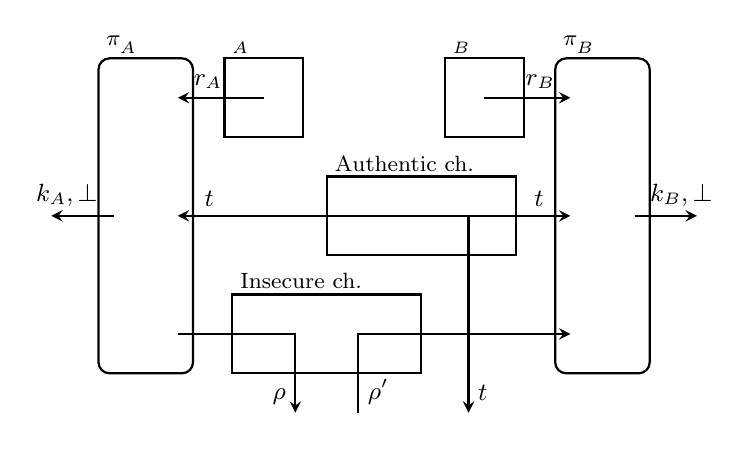
\begin{tikzpicture}[
sArrow/.style={->,>=stealth,thick},
thinResource/.style={draw,thick,minimum width=2.4cm,minimum height=1cm},
pnode/.style={minimum width=.8cm,minimum height=.5cm},
sqResource/.style={draw,thick,minimum width=1cm,minimum height=1cm},
longProtocol/.style={draw,rounded corners,thick,minimum width=1.2cm,minimum height=4cm}]


\small

\def\t{4.1} %.6+1.2+.5+1.2*3/2
\def\u{2.9} %1.2/2+.5+1.2*3/2
\def\v{1.5}
\def\w{.6} %1.2/2
\def\x{.8} %1.2-.4


\node[pnode] (a1) at (-\u,\v) {};
\node[pnode] (a2) at (-\u,0) {};
\node[pnode] (a3) at (-\u,-\v) {};
\node[longProtocol] (a) at (-\u,0) {};
\node[yshift=-2,above right] at (a.north west) {\footnotesize
  $\pi^{\qkd}_A$};
\node (alice) at (-\t,0) {};

\node[pnode] (b1) at (\u,\v) {};
\node[pnode] (b2) at (\u,0) {};
\node[pnode] (b3) at (\u,-\v) {};
\node[longProtocol] (b) at (\u,0) {};
\node[yshift=-2,above right] at (b.north west) {\footnotesize $\pi^{\qkd}_B$};
\node (bob) at (\t,0) {};

\node[sqResource] (ra) at (-\x-\w,\v) {};
\node[yshift=-2,above right] at (ra.north west) {\footnotesize $\aR_A$};
\node[sqResource] (rb) at (\x+\w,\v) {};
\node[yshift=-2,above right] at (rb.north west) {\footnotesize $\aR_B$};
\node[thinResource] (cch) at (\w,0) {};
\node[yshift=-2,above right] at (cch.north west) {\footnotesize
  Authentic ch.~$\aA$};
\node[thinResource] (qch) at (-\w,-\v) {};
\node[yshift=-1.5,above right] at (qch.north west) {\footnotesize
  Insecure ch.~$\aQ$};
\node (eveq1) at (-\w-.4,-\v-1) {};
\node (junc1) at (eveq1 |- a3) {};
\node (eveq2) at (-\w+.4,-\v-1) {};
\node (junc2) at (eveq2 |- a3) {};
\node (evec) at (\w+\w,-\v-1) {};
\node (junc3) at (evec |- b2) {};

\draw[sArrow] (ra.center) to node[auto,swap,pos=.65] {$r_A$} (a1);
\draw[sArrow] (rb.center) to node[auto,pos=.65] {$r_B$}  (b1);

\draw[sArrow,<->] (a2) to node[auto,pos=.08] {$t$} node[auto,pos=.92] {$t$}  (b2);
\draw[sArrow] (junc3.center) to node[auto,pos=.9] {$t$} (evec.center);

\draw[sArrow] (a2) to node[auto,pos=.75,swap] {$k_{A},\bot$} (alice.center);
\draw[sArrow] (b2) to node[auto,pos=.75] {$k_{B},\bot$} (bob.center);

\draw[sArrow] (a3) to (junc1.center) to node[pos=.8,auto,swap] {$\rho$} (eveq1.center);
\draw[sArrow] (eveq2.center) to node[pos=.264,auto,swap] {$\rho'$} (junc2.center) to (b3);

\end{tikzpicture}



\caption[QKD system with explicit randomness
resource]{\label{fig:qkd.real.randomness} A real QKD system with a
  deterministic protocol $(\pi^{\qkd}_A,\pi^{\qkd}_B)$ and explicit
  sources of randomness $\aR_A$ and $\aR_B$.}
\end{figure}

In such a setting, the converters $\pi^{\qkd}_A$ and $\pi^{\qkd}_B$
are deterministic systems. A QKD protocol would then construct an
ideal key resource given access to these three resources. It remains
an open problem to minimize the assumptions on the sources of
randomness in QKD. Recent results on device\-/independent randomness
amplification~\cite{CR12} show that under certain minimal assumptions\footnote{One
  generally has to assume that no messages leave or enter the quantum
  devices unless authorized by the protocol. Some papers make
  additional assumptions to simplify the protocols and proofs.} about
the workings of an unknown quantum system, one can transform a single
(public) weak source of randomness into a fully (private) random
source~\cite{CSW14,BRGHHHSW16,KAF20}. Alternatively, if two (or more)
sources of weak randomness are available to a player (under certain
strict conditions on the correlations between these different
sources), these can be combined to obtain (approximately) uniform
randomness \cite{CLW14,AFPS16}. Composing this with a standard QKD
protocol would allow secret keys to be distributed when only weak
randomness is available to the honest parties.


\subsection{Device-independent QKD}
\label{sec:alternative.di}

In this review we have so far always considered scenarios for which it
is assumed that the players have trusted quantum devices, which work
exactly according to their specifications. For instance, if a player
instructs the device to generate a $\zero$ state, then it is assumed
that the device generates precisely this state. This assumption is
however not met in any actual implementation with realistic devices,
as these are never perfect. Indeed, there have been numerous
demonstrations of successful attacks against implementations of
quantum cryptographic protocols that exploited deviations of the
devices' functionality from the specifications, as discussed in
\secref{sec:attacks}. Crucially, this problem cannot be solved only by
a more careful design of the devices, for it appears to be impossible
to guarantee their perfect working under all possible environmental
conditions.

A theoretical solution to this problem is to devise protocols whose
security does not rely on the assumption that devices are perfect.
Ideally, they should provide security guarantees even if the devices
are untrusted, meaning that their behavior may deviate arbitrarily
from the specification. Remarkably, using quantum devices, this is
possible (with certain caveats described below). The idea is to use a
phenomenon called \emph{(Bell) non\-/locality} \cite{Bell64} \--- see
also \textcite{Sca13,BCPSW14} for review articles on the topic. The
subfield of cryptography that studies the use of non\-/locality to
design protocols that work with untrusted devices is termed
\emph{device\-/independent cryptography}.
  
In a nutshell, a Bell inequality is a bound on the probability of
observing certain values in an experiment involving measurements of two isolated (and hence non-communicating) systems. The bound characterises classical locality: it cannot be violated if
the two isolated systems are described by classical physics. However, the bound can be violated by measurements on entangled quantum systems.   One of the most commonly used Bell inequalities is the
CHSH inequality \cite{CHSH69}. It states that, if two players each
hold non\-/communicating systems, and each performs one out of two
binary measurements chosen uniformly at random on their respective
system, where the choice of the measurement is given by
$x,y \in \{0,1\}$ and the outcome is given by $a,b \in \{0,1\}$,
respectively, then the probability that $xy = a \xor b$ should be less than
or equal to $3/4$.\footnote{An alternative formulation of the
  inequality is
  $\left| E(0,0) + E(0,1) + E(1,0) - E(1,1) \right| \leq 2$, where
  $E(x,y)$ is the expected value of the product of the outcomes of the
  systems when measured with settings $x$ and $y$, respectively, and
  the outcomes are values in $\{-1,+1\}$.} But if the systems are
quantum, it is possible to observe this outcome with probability up to
$\approx .85$ \--- this is achieved if the systems are in a perfectly
entangled state and the players perform an optimal measurement.

An observation of a violation of a Bell inequality implies that the
measurement outcomes contain some genuine randomness
\cite{Col06,PAM10,AMP12,CR12}, even conditioned on the knowledge of
the person who set up and programmed the devices used in the
experiment \--- the only assumptions being that no information other
than the measurement result leaves the devices, and that these devices
never fall in the hands of an adversary, since their internal memory
may contain a copy of the measurement outcomes. This randomness may
then be used to generate uniform random numbers
\cite{VV12,CSW14,MS14,BRGHHHSW16,KAF20} or a shared secret key
\cite{BHK05,PABGMS09,VV14,ADFRV18,AFRV19}.

For a review of different results and techniques in
device\-/independent cryptography, we refer to \textcite{ER14}. In
this section we show how to model device\-/independent quantum key
distribution (DI-QKD) in the AC framework. It then follows from the
composition theorem of AC, that the resulting key can be safely used
in applications requiring one.

The converters $\pi^\qkd_A$ and $\pi^\qkd_B$ modeling Alice's and
Bob's parts of the protocol in \secref{sec:qkd} are systems which
generate quantum states and perform measurements. In DI-QKD, exactly
these operations cannot be trusted. So instead, the DI protocol
$(\pi^\diqkd_A,\pi^\diqkd_B)$ will only involve \emph{classical}
operations. Everything \emph{quantum} is moved into a resource, a
device $\aD$. The honest players can send bits to these devices, and
receive bits back from them \--- this corresponds to choosing a
measurement $x,y \in \{0,1\}$ and receiving the outcome
$a,b \in \{0,1\}$, described a few paragraphs earlier. The adversary is
permitted to ``program'' these devices by providing some initial state
$\rho$ as input \--- depending on the model, Eve may be allowed to
provide further inputs to the device at some later point, e.g., to
provide more EPR pairs so that it may continue running. The
corresponding real world is drawn in
\figref{fig:alternatives.diqkd}. The ideal world will be identical to
that of standard QKD, since we wish to construct the same key
resource, i.e., \figref{fig:qkd.resource.sim}.


\begin{figure}[tb]

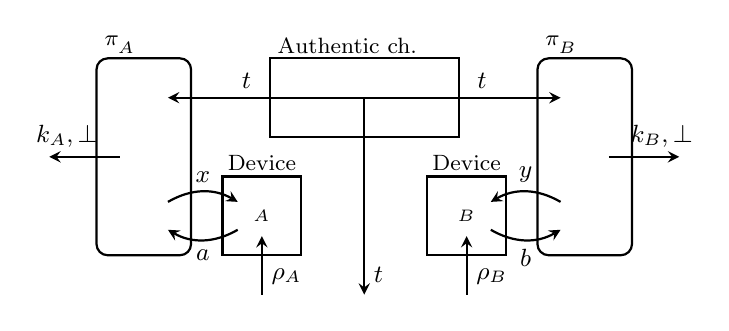
\begin{tikzpicture}[
sArrow/.style={->,>=stealth,thick},
thinResource/.style={draw,thick,minimum width=2.4cm,minimum height=1cm},
sqResource/.style={draw,thick,minimum width=1cm,minimum height=1cm},
protocol/.style={draw,rounded corners,thick,minimum width=1.2cm,minimum height=2.5cm},
pnode/.style={minimum width=.6cm,minimum height=.5cm}]

\small

\def\t{4} %.6+1.2+.4+1.2*3/2
\def\u{2.8} %1.2/2+.4+1.2*3/2
\def\v{.75}
\def\w{1.3} 

\node[pnode] (a1) at (-\u,\v) {};
\node[pnode] (a2) at (-\u,0) {};
\node[pnode] (a3) at (-\u,-\v) {};
\node[protocol] (a) at (-\u,0) {};
\node[yshift=-2,above right] at (a.north west) {\footnotesize
  $\pi^{\diqkd}_A$};
\node (alice) at (-\t,0) {};

\node[pnode] (b1) at (\u,\v) {};
\node[pnode] (b2) at (\u,0) {};
\node[pnode] (b3) at (\u,-\v) {};
\node[protocol] (b) at (\u,0) {};
\node[yshift=-2,above right] at (b.north west) {\footnotesize $\pi^{\diqkd}_B$};
\node (bob) at (\t,0) {};

\node[thinResource] (cch) at (0,\v) {};
\node[yshift=-2,above right] at (cch.north west) {\footnotesize
  Authentic ch.~$\aA$};
\node[sqResource] (da) at (-\w,-\v) {$\aD_A$};
\node[yshift=-1.5,above] at (da.north) {\footnotesize
  Device};
\node[pnode] (dan) at (-\w,-\v) {};
\node[sqResource] (db) at (\w,-\v) {$\aD_B$};
\node[yshift=-1.5,above] at (db.north) {\footnotesize
  Device};
\node[pnode] (dbn) at (\w,-\v) {};

\node (eveq1) at (-\w,-1.75) {};
\node (eveq2) at (\w,-1.75) {};
\node (evec) at (0,-1.75) {};
\node (junc3) at (evec |- b1) {};

\draw[sArrow,<->] (a1) to node[auto,pos=.2] {$t$} node[auto,pos=.8] {$t$}  (b1);
\draw[sArrow] (junc3.center) to node[auto,pos=.9] {$t$} (evec.center);

\draw[sArrow] (a2) to node[auto,pos=.75,swap] {$k_{A},\bot$} (alice.center);
\draw[sArrow] (b2) to node[auto,pos=.75] {$k_{B},\bot$} (bob.center);

\draw[sArrow] (eveq1.center) to node[pos=.3,auto,swap] {$\rho_A$} (dan);
\draw[sArrow] (eveq2.center) to node[pos=.3,auto,swap] {$\rho_B$} (dbn);

\draw[sArrow,bend left] (a3) to node[pos=.5,auto] {$x$} (dan);
\draw[sArrow,bend left] (dan) to node[pos=.5,auto] {$a$} (a3);
\draw[sArrow,bend right] (b3) to node[pos=.5,auto,swap] {$y$} (dbn);
\draw[sArrow,bend right] (dbn) to node[pos=.5,auto,swap] {$b$} (b3);

\end{tikzpicture}


\caption[DI-QKD]{\label{fig:alternatives.diqkd}The real world setting
  for  a DI-QKD protocol. Eve can program the devices $\aD$, but cannot
  receive any output from them.}
\end{figure}

Applying \defref{def:security}, this means that the protocol
$(\pi^\diqkd_A,\pi^\diqkd_B)$ constructs $\aK$ from $\aA$, $\aD_A$ and
$\aD_B$ within $\eps$ if
\begin{equation} \label{eq:diqkd}
  \exists \sigma_E, \quad \pi_A^{\diqkd}\pi_B^{\diqkd}(\aD_A \| \aD_B \| \aA)
  \close{\eps} \aK \sigma_E.
\end{equation}
Note that we have not specified the behaviors of the devices $\aD_A$
and $\aD_B$ at all. In fact, we need \eqnref{eq:diqkd} to hold for all
devices $\aD_A$ and $\aD_B$.\footnote{The simulator may depend on
  these devices, i.e., $\forall \aD_A, \aD_B, \exists \sigma_E$ such
  that \eqnref{eq:diqkd} holds.} This is exactly the
\emph{device\-/independant} guarantee, namely that security holds
regardless of how the (quantum) devices work. Alternatively one can
consider fixed devices $\aD_A$ and $\aD_B$ that are universal
computers, and have their program be part of the inputs at the $E$ interface.

As usual, completeness is captured by specific devices $\aD'_A$ and
$\aD'_B$ that work honestly \--- e.g., they share perfectly entangled
states and perform the correct measurements as specified by the
protocol \--- as well as the same honest resources $\aA'$ and $\aK'$
as in \secref{sec:qkd}. Additionally to
\eqnref{eq:diqkd}, we also need
\begin{equation*} %\label{eq:qkd.robust}
  \pi_A^{\diqkd}\pi_B^{\diqkd}(\aD'_A \| \aD'_B
  \| \aA') \close{\eps'} \aK'.
\end{equation*}

The same reduction as for (normal) QKD goes through, and one can show
that \eqnref{eq:diqkd} is satisfied if for all behaviors of the
devices (and their inputs), \eqnsref{eq:qkd.cor} and \eqref{eq:qkd.sec}
hold.

Note however that the construction outlined in this section only
allows the devices $\aD_A$ and $\aD_B$ to be accessed during the
protocol. No access is granted after the protocol ends, meaning that
we make no security statement about what happens if the devices are
reused. It is an open question how to reuse devices in DI
cryptography, which we discuss in \secref{sec:open.di}.

Proving security of device-independent QKD is more challenging than in
the device-dependent case. One of the difficulties is that the
measurement operators that describe Alice and Bob's measurement can be
arbitrary. In particular it cannot be assumed, for instance, that two
subsequent measurement outcomes by Bob are obtained by two separate
measurement processes. While some of the techniques described
in~\secref{sec:securityproofs}, such as entropy accumulation, are
still applicable to the device-independent setting, others, like de
Finetti-type theorems, are not or must be adapted,
[see~\textcite{ArnonThesis} for details].

\subsection{Semi-device-independent QKD}
\label{sec:alternative.semi}

The only assumption made about the devices in DI-QKD is that no
information leaves these devices unless allowed by the protocols (see
\secref{sec:alternative.di}). But achieving the violation of Bell
inequalities needed for this is challenging because it requires high
detector efficiency and tolerates only low noise on the
channel~\cite{BCPSW14}. Protocols that are easier to implement can be
achieved by making additional assumptions about the quantum devices
used by Alice and Bob. These are generally called
\emph{semi\-/device\-/independent} (semi-DI).

Many different assumptions may be labeled semi-DI. For example, in a
one-sided device-independent setting the protocol is DI for Bob but
not for Alice \cite{BCWSW12}. One may also assume dimension bounds on
the quantum systems generated by untrusted devices as in
\textcite{PB11}. Alternatively, \textcite{LPTRG13} assume that each
use of the devices are causally independent \--- i.e., the states
generated and measurements performed are in product form \--- to
analyze a protocol where the Bell violation is measured locally in
Alice's lab, thus avoiding the noise introduced by the channel between
Alice and Bob. Similar ideas have been used for other protocols than
QKD, e.g., semi-DI quantum money~\cite{HS20,BDG19}.

One of the most promising forms of semi-DI QKD, which has already been
implemented over large distances
\cite{Liu13,Tang2014,Pirandola2015,Yin2016} is
\emph{measurement\-/device\-/independent} (MDI) QKD
\cite{LCQ12,BP12,MR12,CXCLTL14}. Here, one assumes that players can
generate the states they desire, but one does not trust measurement
devices at all. This model is motivated by the attacks on the
detectors, e.g., the time-shift attacks or detector blinding attacks
discussed in \secref{sec:attacks:hacking}.

To understand how such protocols work, we will start from an
entanglement based protocol as in
\secref{sec:alternative.entanglement}, then modify it step by
step, until we achieve a prepare\-/and\-/measure protocol, in which
all measurements are performed by the adversary. Since the final
protocol is as secure as the original one, and the original one is
secure for all adversaries, the final MDI QKD protocol is secure
for all adversaries as well. In particular, it is secure for
adversaries that completely control the measurement apparatus.

In an entanglement based protocol, Alice and Bob receive the $A$ and
$B$ parts of a state $\psi_{ABR}$, and measure these systems in either
the computational or diagonal basis, obtaining a raw key. This key is
then processed as in a prepare\-/and\-/measure protocol (see
\secref{sec:qkd.protocol} and \secref{sec:securityproofs}).  If the
source gave them a state which is (close to) a tensor product of EPR
pairs, such a protocol is guaranteed to terminate with a shared secret
key. Equivalently, the source could generate any of the Bell states,
and notify Alice and Bob which one it gave them. They then perform bit
or phase flips to change it to an EPR pair.

Instead of the source distributing an entangled state, Alice and Bob
could each generate an EPR pair $AA'$ and $BB'$, respectively. They
then send $A'$ and $B'$ to a third party, Charlie, who measures this
in the Bell basis, and tells them the measurement outcome. If
performed correctly, the $AB$ system will be in a Bell state, and the
measurement outcome will tell them which one. By flipping bits or
phases, Alice and Bob can turn this into an EPR pair, and continue
with the protocol as above. Crucially, if Charlie does not perform the
correct measurement, then Alice and Bob will end up holding the $A$
and $B$ parts of some unknown state $\psi_{ABR}$. But this does not
compromise security: if it is too far from the expected state, the
protocol will just abort.

Instead of first performing a bit or phase flip, and then measuring,
Alice and Bob could first measure their systems $A$ and $B$, and then
flip the value of the measurement outcome if needed. And instead of
generating EPR pairs $AA'$ and $BB'$, then measuring $A$ and $B$, they
could pick the measurement outcome at random, then generate the
corresponding reduced state in $A'$ and $B'$ respectively, send these
to Charlie, and when they obtain the measurement outcome from Charlie,
they flip their bits if needed.

The only (trusted) quantum operations that Alice and Bob need to
perform in the protocol described in the paragraph above are
generating the states in the systems $A'$ and $B'$. All measurements
have now been delegated to Charlie, who may deviate arbitrarily from
the protocol without compromising security.

The real world for such a MDI-QKD protocol is drawn in
\figref{fig:alternatives.mdi}, where one can see that the converters
$\pi^{\mdi}_A$ and $\pi^{\mdi}_B$ do not have any incoming quantum
states, i.e., they do not need to perform any measurement.

Security proofs for MDI-QKD protocols can be based on the same techniques as those for fully device-independent protocols, as discussed in \secref{sec:alternative.di}. The comments on security proofs made in that section thus also apply here. 

\begin{figure}[tb]

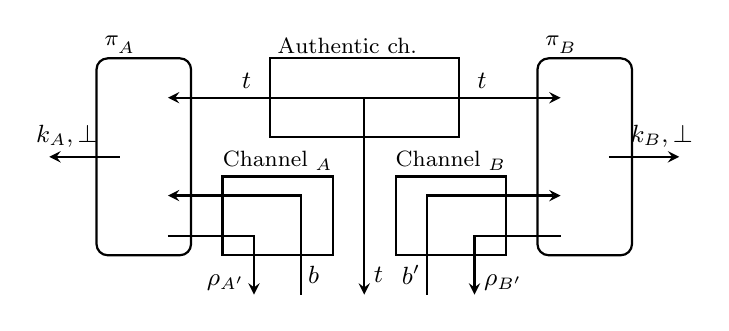
\begin{tikzpicture}[
sArrow/.style={->,>=stealth,thick},
thinResource/.style={draw,thick,minimum width=2.4cm,minimum height=1cm},
sqResource/.style={draw,thick,minimum width=1.4cm,minimum height=1cm},
protocol/.style={draw,rounded corners,thick,minimum width=1.2cm,minimum height=2.5cm},
pnode/.style={minimum width=.6cm,minimum height=.5cm}]

\small

\def\t{4} %.6+1.2+.4+1.2*3/2
\def\u{2.8} %1.2/2+.4+1.2*3/2
\def\v{.75}
\def\w{1.1} 
\def\a{.3}

\node[pnode] (a1) at (-\u,\v) {};
\node[pnode] (a2) at (-\u,0) {};
\node[pnode] (a3) at (-\u,-\v) {};
\node[protocol] (a) at (-\u,0) {};
\node[yshift=-2,above right] at (a.north west) {\footnotesize
  $\pi^{\mdi}_A$};
\node (alice) at (-\t,0) {};

\node[pnode] (b1) at (\u,\v) {};
\node[pnode] (b2) at (\u,0) {};
\node[pnode] (b3) at (\u,-\v) {};
\node[protocol] (b) at (\u,0) {};
\node[yshift=-2,above right] at (b.north west) {\footnotesize $\pi^{\mdi}_B$};
\node (bob) at (\t,0) {};

\node[thinResource] (cch) at (0,\v) {};
\node[yshift=-2,above right] at (cch.north west) {\footnotesize
  Authentic ch.~$\aA$};
\node[sqResource] (da) at (-\w,-\v) {};
\node[yshift=-1.5,above] at (da.north) {\footnotesize
  Channel $\aC_A$};
\node[pnode] (dan) at (-\w,-\v) {};
\node[sqResource] (db) at (\w,-\v) {};
\node[yshift=-1.5,above] at (db.north) {\footnotesize
  Channel $\aC_B$};
\node[pnode] (dbn) at (\w,-\v) {};

\node (eveq11) at (-\w-\a,-1.75) {};
\node (eveq12) at (-\w+\a,-1.75) {};
\node (eveq21) at (\w-\a,-1.75) {};
\node (eveq22) at (\w+\a,-1.75) {};
\node (evec) at (0,-1.75) {};
\node (junc3) at (evec |- b1) {};

\draw[sArrow,<->] (a1) to node[auto,pos=.2] {$t$} node[auto,pos=.8] {$t$}  (b1);
\draw[sArrow] (junc3.center) to node[auto,pos=.9] {$t$} (evec.center);

\draw[sArrow] (a2) to node[auto,pos=.75,swap] {$k_{A},\bot$} (alice.center);
\draw[sArrow] (b2) to node[auto,pos=.75] {$k_{B},\bot$} (bob.center);

\draw[sArrow] (a3.south east) to (eveq11 |- a3.south east) to node[pos=.8,auto,swap] {$\rho_{A'}$} (eveq11.center);
\draw[sArrow] (b3.south west) to (eveq22 |- b3.south west) to node[pos=.8,auto] {$\rho_{B'}$} (eveq22.center);
\draw[sArrow] (eveq12.center) to node[pos=.2,auto,swap,xshift=-1] {$b$} (eveq12 |- a3.north east) to (a3.north east);
\draw[sArrow] (eveq21.center) to node[pos=.2,auto,xshift=1] {$b'$} (eveq21 |- b3.north west) to (b3.north west);

\end{tikzpicture}


\caption[MDI-QKD]{\label{fig:alternatives.mdi}The real world setting
  for a MDI-QKD protocol. The only quantum operations performed by
  $\pi^{\mdi}_A$ and $\pi^{\mdi}_B$ are the generation of quantum
  states. The communication resources $\aC$ send quantum systems from
  Alice or Bob to Eve, and classical bits from Eve to Alice and Bob..}
\end{figure}

\subsection{Memoryless adversaries}
\label{sec:alternative.memoryless}

The previous sections analyzed different models of QKD, in which we
changed the capabilities and resources of the honest players running
the protocol. Similar techniques may also be used to model
limitations on adversaries. In this last section we consider as example QKD
protocol with an adversary that has no (long-term) quantum memory, and is
forced to measure the quantum states exchanged between Alice and Bob
during the QKD protocol and store the classical information.

The insecure channel resource, $\aQ$, modeled as part of the real QKD
system in \figref{fig:qkd.real.adv} gives complete control over the
states sent on this channel to the adversary. Since this may include
storing them and measuring them at a later point, we need to limit the
adversary's access to this channel as part of the insecure channel
resource. We may thus define a different channel $\tilde{\aQ}$, which
requires Eve to input some measurement specification and then obtains
the measurement outcome at her interface. The resulting
post\-/measurement state is then output at Bob's interface.

The model of $\tilde{\aQ}$ described above is just one possible way
one may imagine limiting Eve's access to the states sent during
QKD. The result is a change in the requirements of the QKD
protocol. Instead of constructing a secure key $\aK$ from an authentic
channel $\aA$ and an insecure channel $\aQ$, it is now sufficient if
$\aK$ can be constructed from $\aA$ and $\tilde{\aQ}$. It is not hard
to see that, since the accessible information (see
\secref{sec:qkd.other.ai}) measures the information an adversary has
\emph{after} measuring their quantum states, a QKD protocol with low
accessible information would satisfy such a construction \--- namely,
$\aA \| \tilde{\aQ} \rightarrow \aK$. The accessible information
security measure is thus a composable criterion under the assumption
that the adversary has such a physical limit on their memory.

Since QKD protocols are secure against general adversaries as modeled
in \secref{sec:qkd}, there does not seem to be much incentive to
consider adversaries with limitations on their memory (unlike for some
two-party protocols discussed in \secref{sec:open.other}). It is
however noteworthy that, as already mentioned in
\secref{sec:qkd.other.ac}, by explicitly limiting the adversary's
capabilities we capture weaker security notions that appeared in the literature.


%%% Local Variables:
%%% TeX-master: "main.tex"
%%% End:
